% =============================================================================
% AmphionASR 2.0: Target-Speaker Speech Recognition for Real-World Recordings --- A Benchmark and a Model — built with Amphion PaperKit
% Uses the public LaTeX template shipped with Amphion PaperKit
% (template/amphion.cls). Default theme = amphion (warm ivory + petrol teal);
% see template/CHANGELOG.md for available [opendfm] / [xlance] / [withlogo]
% options.
%
% Placeholders use the <<NAME>> form (angle brackets, LaTeX-safe). Run
% tools/new-report.sh <slug> to substitute them automatically.
% =============================================================================

\documentclass{template/amphion}

% --- ASR-domain math macros (\wer / \cer / \mer / \hotwerN). Drop if not ASR.
\usepackage{template/asr-macros}

% --- Report-wide names. The benchmark name is tentative (refs/docs/plan.md §4);
%     renaming it is a one-line change here.
\newcommand{\tsbench}{AmphionTS-Bench\xspace}
\newcommand{\septok}{\texttt{[SEP]}\xspace}

% --- PDF metadata (theme + page styles owned by template/amphion.cls) -------
\hypersetup{
  pdftitle={AmphionASR 2.0: Target-Speaker Speech Recognition for Real-World Recordings --- A Benchmark and a Model},
  pdfsubject={cs.CL},
  pdfauthor={Amphion Team},
  pdfkeywords={Target-speaker ASR, Benchmark, SpeechLLM},
}

% --- Title, author, abstract ------------------------------------------------
\title{AmphionASR 2.0: Target-Speaker Speech Recognition for Real-World Recordings --- A Benchmark and a Model}
\author{Amphion Team}
\abstract{% Abstract — supplied to \abstract{} in main.tex (no environment).
% Jobs, one per sentence (paper-writing.mdc §2; refs/docs/plan.md §5):
% task -> gap -> benchmark + key contrast -> model -> headline + retention.
% Numbers: refs/internal/html-report/data.json (v12.headline, supp.bench, asr).

Target-speaker automatic speech recognition (TS-ASR) transcribes only the person heard in a few seconds of enrollment speech and should output nothing when that person does not speak.
It was the capability of AmphionASR~1.0 that most needed work.
Common evaluations mix read utterances, always contain the target, and score only target-present samples, so they cannot measure the most common error in real use: transcribing someone else while the enrolled speaker is silent.
We propose \tsbench, a Mandarin benchmark of 24{,}101 samples in 248 subsets, to be released publicly.
It pairs every condition with target-present and target-absent samples and adds real meeting, phone-call and web-conversation recordings without mixing.
On this benchmark, two systems with almost the same character error rate (CER) when only the target talks in real recordings (7.5\% and 7.3\%) have false-alarm rates of 2.6\% and 96.1\% on real recordings in which others talk.
We also present AmphionASR~2.0, a 1.7\,B SpeechLLM fine-tuned from Qwen3-ASR-1.7B.
It joins the enrollment and the mixture with a learnable separator inside its audio encoder, and every scene type in its training data has target-absent counterparts.
On \tsbench it reaches 13.1\% CER on target-present samples and a 3.7\% false-alarm rate on target-absent samples, against 33.4\% and 67.8\% for Xiaomi-CocktailASR-1, a model about five times larger.
The same weights are 0.1 to 1.0 points behind Qwen3-ASR-1.7B on the category means of public plain-ASR test sets.
}
% TODO: replace with the AmphionTS-Bench / model release link once decided
% (refs/docs/plan.md §4.3); the scaffold default is kept until then.
\metadatainfo{
  \small\makebox[\linewidth][c]{
    \href{https://github.com/amphionspace/technical-reports}{\texttt{GitHub: amphionspace/technical-reports}}
  }
}

% =============================================================================
\begin{document}
\publishdate{2026.10.31}
\maketitle

% --- Body page header: short name (full \title is too long for every page) --
\fancyhead[L]{AmphionASR 2.0}

\clearpage
\tableofcontents
\clearpage

% --- Relax float placement so tables share pages with text (as in 1.0) ------
\renewcommand{\topfraction}{0.92}
\renewcommand{\textfraction}{0.05}
\renewcommand{\floatpagefraction}{0.7}
\setcounter{topnumber}{3}

% --- Body sections ----------------------------------------------------------
% Introduction. Source: HTML §1 (refs/internal/html-report/amphionasr-report-en.html);
% 1.0 facts: AmphionASR 1.0 PDF §5.4 (amphion2026amphionasr).
% Structure modelled on the 1.0 report's introduction (problem scenario ->
% shortfall -> contributions), per AGENTS.md rule 6.

\section{Introduction}
\label{sec:intro}

\begin{figure}[t]
  \centering
  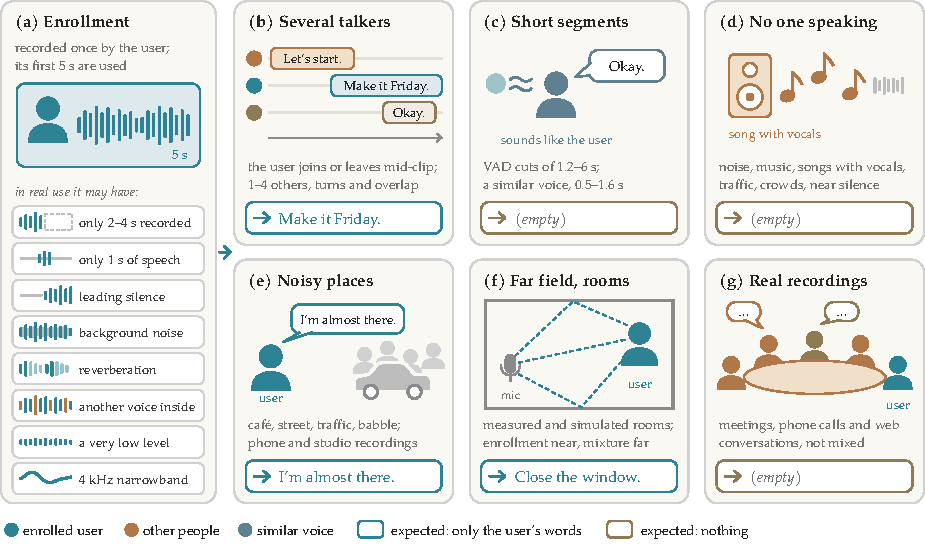
\includegraphics[width=\linewidth]{figures/scenarios.pdf}
  \caption{Situations from real use that \tsbench covers, one panel per section of the benchmark. (a)~The enrollment, recorded once by the user, of which the first 5\,s are used, and the degradations it may have in real use. (b)--(g)~Situations in the recording, each with the output expected from a TS-ASR model: only the enrolled user's words, or nothing when the user does not speak. VAD: voice activity detection. Utterances are illustrative; the benchmark is in Mandarin.}
  \label{fig:scenarios}
\end{figure}

\begin{figure}[t]
  \centering
  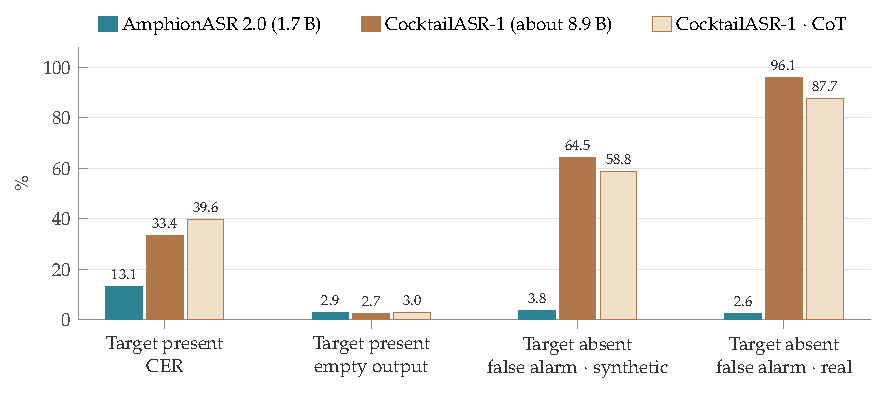
\includegraphics[width=\linewidth]{figures/main-results.pdf}
  \caption{Main results on \tsbench (\%, lower is better). The first two metric groups are computed on target-present samples only; the two false-alarm groups are computed on target-absent samples only, from synthetic scenes and from real meetings, calls and web conversations. All systems use the same audio, the first 5\,s of each enrollment and the same scoring.}
  \label{fig:teaser}
\end{figure}

SpeechLLMs connect an audio encoder to an autoregressive language model and are now used as general-purpose speech recognizers~\cite{shi2026qwen3asr}.
In meetings, at reception desks, in cars and on the street, however, a recording often contains several people speaking at once or in turn, and the user usually cares about only one of them.
Target-speaker automatic speech recognition (TS-ASR) addresses this case: the model receives an enrollment utterance of one person together with the recording, called the mixture, and transcribes only what that person says.
The task has two kinds of error that pull in opposite directions.
A \emph{miss} occurs when the enrolled speaker spoke but the model wrote nothing or only part of it; a \emph{false alarm} occurs when the enrolled speaker did not speak but the model transcribed someone else.
\Cref{fig:scenarios} shows the situations from real use covered by our benchmark, \tsbench; the correct output is either the enrolled user's words or nothing at all.

Our earlier AmphionASR~1.0~\cite{amphion2026amphionasr} combined retrieval-augmented hotwords, target-speaker selection, degradation robustness and whispered speech in one 1.7\,B model, and of these capabilities TS-ASR most needed work.
Its in-house test set was synthesized in the same way as its target-speaker training data.
That report gives a target-present WER of 13.02\%, measures the target-absent case only on 164 samples in which nobody speaks, and does not test what the model does when others speak while the enrolled speaker is silent.
The 1.0 report itself notes that these results do not establish competitiveness with dedicated TS-ASR systems under a matched protocol~\cite{amphion2026amphionasr}.
AmphionASR~2.0 therefore takes TS-ASR as its main target.

Improving TS-ASR first requires an evaluation that reflects real use.
Common evaluations of target speech extraction (TSE) and TS-ASR, such as WSJ0-2mix~\cite{hershey2016deep}, Libri2Mix~\cite{cosentino2020librimix} and LibriSpeechMix~\cite{kanda2020serialized}, overlay two or three read utterances.
The target is always present, the enrollment is another clean utterance of the same person, and metrics are computed only on target-present samples~\cite{zmolikova2019speakerbeam, zmolikova2023neural}.
WHAM!~\cite{wichern2019wham} and WHAMR!~\cite{maciejewski2020whamr} add noise and reverberation but keep the same mixing, and SpeechLLM work on TS-ASR mostly reports error rates on synthetic two-talker mixtures~\cite{zhang2025thinking, guo2024sqwhisper}.
These evaluations differ from real use in three ways:
\begin{itemize}[leftmargin=*, itemsep=2pt]
  \item \textbf{False alarms go unmeasured.} Without target-absent samples, a model that transcribes everyone can still score well; TSE research has also shown that evaluations assuming an always-active target hide false extractions~\cite{delcroix2022listen}.
  \item \textbf{No conversational structure.} Randomly overlaid read sentences lack the turn-taking, interjections, hand-overs, simultaneous starts and one- or two-word replies of meetings and conversations.
  \item \textbf{No real enrollment or recording conditions.} A user's enrollment may be short, noisy or contain another voice, and the recording may come from a far-field microphone or a phone call.
\end{itemize}

This report makes two contributions:
\begin{itemize}[leftmargin=*, itemsep=2pt]
  \item \textbf{\tsbench, a TS-ASR benchmark for real-world conditions} (\Cref{sec:benchmark}). It pairs every condition with target-present and target-absent samples and reports three metrics together. Its synthetic scenes are designed from errors observed in real use and change one factor at a time. Its real part comes from the test sets of public meeting and call corpora and from web conversations, without mixing. With 24{,}101 samples in 248 subsets, it shows that evaluations limited to a single talker, to samples with the target present or to silence lead to conclusions that do not hold in real conditions (\Cref{subsec:exp_conditions}). The benchmark will be released publicly.
  \item \textbf{AmphionASR~2.0, a TS-ASR model that also keeps plain and hotword recognition} (\Cref{sec:model,sec:data,sec:training}). The enrollment and the mixture pass separately through the convolutional downsampling of the audio encoder and are joined by a learnable separator before its Transformer layers, which attend globally. The training data are organized by scene type, each with target-absent counterparts that enroll another person, and include real meeting windows. Compared with Xiaomi-CocktailASR-1~\cite{zhang2026xiaomi} on \tsbench under the same protocol, AmphionASR~2.0 has about two fifths of its target-present CER and a false-alarm rate more than an order of magnitude lower when others talk and the enrolled speaker is silent (\Cref{fig:teaser}).
\end{itemize}

AmphionASR~2.0 is also initialized from Qwen3-ASR-1.7B~\cite{shi2026qwen3asr} but differs from 1.0 in two ways: all of its parameters are fine-tuned, and the enrollment is placed inside the audio encoder.
In 1.0, the enrollment is encoded separately and enters the language model as its own span of audio embeddings.
Version~2.0 does not include the hotword-retrieval module or the whispered-speech training of 1.0, and this report does not evaluate those two capabilities.

% AmphionTS-Bench. Sources: refs/docs/ts_benchmark.md §1--4; HTML §2 (tables 1--2).
% Counts verified against the AmphionEval records of the v12 benchmark
% (248 subsets, 12,950 present / 11,151 absent).

\section{\tsbench: A TS-ASR Benchmark for Real-World Conditions}
\label{sec:benchmark}

\tsbench aims to make evaluation scores agree with behavior in real use.
It is a Mandarin benchmark with a synthetic part and a real part, and it will be released publicly.
\Cref{tab:bench_vs_common} contrasts it with common evaluations, and \Cref{fig:bench} shows how its samples are built.

\begin{figure}[t]
  \centering
  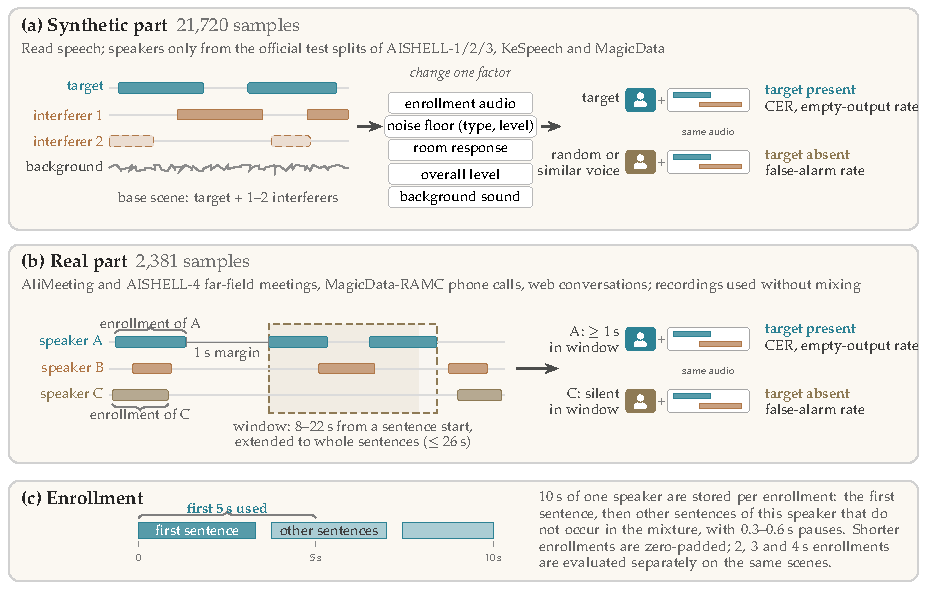
\includegraphics[width=\linewidth]{figures/bench-construction.pdf}
  \caption{Construction of \tsbench. (a)~Synthetic part: on base scenes of the target and one or two interferers (dashed: the second interferer), one factor is changed at a time. (b)~Real part: recordings are cut into windows without mixing, and the enrollment comes from the same recording outside the window. In both parts, every mixture yields a target-present and a target-absent sample with identical audio that differ only in the enrollment; for the absent sample it belongs to a random person or to one of the five speakers closest to an interferer (synthetic), or to a speaker of the same recording who is silent in the window (real). (c)~Each enrollment stores 10\,s of one speaker, and the first 5\,s are used.}
  \label{fig:bench}
\end{figure}

\begin{table}[t]
  \caption{\tsbench compared with common TSE and TS-ASR evaluations.}
  \label{tab:bench_vs_common}
  \centering
  \small
  \begin{tabularx}{\linewidth}{@{}l>{\raggedright\arraybackslash}p{3.6cm}>{\raggedright\arraybackslash}X@{}}
    \toprule
     & Common evaluations & \tsbench \\
    \midrule
    Speech & Synthetic mixtures of read speech & Synthetic mixtures of read speech; real meeting, phone-call and web-conversation recordings, not mixed \\
    Talkers & 2--3 & 0--5 in the synthetic part; real windows split into 1, 2 and 3+ talkers \\
    Target presence & Always present & Every condition has present and absent groups; 11{,}151 absent samples \\
    Timing & Utterances overlaid with random delays & Continuous speech, interjections, mid-clip entry or exit, turn-taking, simultaneous starts, hand-overs, about 1\,s of speech \\
    Enrollment & Another clean utterance of the same person & First 5\,s; only 2--4\,s recorded, only 1\,s of speech, leading silence, narrowband, noise, reverberation, another voice mixed in, very quiet; enrollments from real meetings \\
    Acoustics & Clean, or with synthetic noise and reverberation & Real ambient noise floors, measured and simulated room responses, near-field and far-field mismatch, level and recording chain, babble and environmental events \\
    Nobody speaking & Usually absent & Noise, music, traffic, near silence, babble, crowds, songs with vocals \\
    Metrics & SDR or WER with the target present & Target-present CER and empty-output rate, target-absent false-alarm rate \\
    \bottomrule
  \end{tabularx}
  \par\smallskip
  {\footnotesize Common evaluations are test sets synthesized from read speech, such as WSJ0-2mix~\cite{hershey2016deep}, Libri2Mix~\cite{cosentino2020librimix}, WHAM!~\cite{wichern2019wham}, WHAMR!~\cite{maciejewski2020whamr} and LibriSpeechMix~\cite{kanda2020serialized}; their exact settings vary.\par}
\end{table}

\subsection{Design principles}
\label{subsec:bench_principles}

\paragraph{Both kinds of error are scored.}
Every condition has a target-present and a target-absent group, and the 11{,}151 absent samples make up nearly half of the benchmark.
Present samples report CER and the empty-output rate, and absent samples report the false-alarm rate.
The three metrics must be read together: a model that merely suppresses false alarms also drops the enrolled speaker's speech, which appears as a higher empty-output rate.

\paragraph{Scenes come from errors observed in real use.}
Each subset corresponds to a specific failure hypothesis rather than a random combination of conditions.
During continuous listening, for example, voice activity detection may cut a 1.2--6\,s segment in which only someone else speaks.
Other examples are the enrolled speaker finishing a sentence and another person replying with a sentence that starts the same way, a similar-sounding person saying one short phrase of 0.5--1.6\,s, only a song with vocals playing, and a user who spoke for only 2--4\,s when enrolling.

\paragraph{Paired, single-factor conditions.}
The synthetic part draws scenes, enrollments and backgrounds from three independent random streams.
Each base scene has the target and one or two interferers.
On these scenes, a single factor is changed at a time: the enrollment audio, the type and level of the noise floor, the room response, the overall level or the background sound.
Absent samples are paired as well: the mixture is identical item by item, and only the enrollment changes.
The new enrollment belongs to a random person or to one of the five speakers whose embeddings are closest to an interferer in the mixture.
Differences between such conditions are therefore paired differences in that one factor.

\paragraph{Real recordings without mixing.}
The real part comes from the human-annotated test sets of the AliMeeting~\cite{yu2022m2met} and AISHELL-4~\cite{fu2021aishell4} far-field meetings (first array channel) and the MagicData-RAMC~\cite{yang2022open} phone calls, plus multi-party web conversations from Emilia~\cite{he2024emilia} with pseudo-labels.
A window starts at the beginning of a sentence, spans 8--22\,s, and is extended to include every complete sentence that overlaps it, up to 26\,s; windows do not overlap.
Each window yields a target-present sample, for someone who speaks for at least 1\,s in it, and a target-absent sample with identical audio.
The absent sample enrolls someone from the same recording who does not speak in the window or, if there is no such person, a speaker from another recording of the same corpus.
The enrollment is taken from the same recording outside the window, with a 1\,s margin.
The same AliMeeting windows also come in four combinations of near-field (headset) and far-field audio for the enrollment and the mixture, which we use to calibrate the synthetic far-field conditions (\Cref{subsec:exp_conditions}).

\paragraph{An enrollment protocol matched to deployment.}
Each enrollment stores 10\,s of the same speaker: the first sentence is followed by other sentences of this person that do not occur in the mixture, with 0.3--0.6\,s pauses between them.
As in deployment, the first 5\,s are used at evaluation time, and shorter enrollments are zero-padded.
Enrollments of only 2, 3 or 4\,s are evaluated separately on the same scenes.

\paragraph{Speaker splits and label checks.}
Synthetic speakers come only from the official test splits of AISHELL-1~\cite{bu2017aishell1}, AISHELL-2~\cite{du2018aishell2}, AISHELL-3~\cite{shi2021aishell3}, KeSpeech~\cite{tang2021kespeech} and MagicData.
In the real windows, presence and absence follow the human-annotated utterance timeline.
Samples whose first 5\,s of enrollment contain at least 0.3\,s of another speaker are reported separately as ``enrollment contains another voice'' and are not scored as clean enrollments.
We also checked with speaker embeddings that each enrollment really belongs to the target, replaced three AISHELL-4 enrollments that belonged to another participant, and removed one window whose target could not be confirmed.

\subsection{Composition}
\label{subsec:bench_composition}

\Cref{tab:bench_composition} lists the size of each section.
The synthetic part has 21{,}720 samples and the real part 2{,}381; each synthetic subset has 120 or 150 samples, and the real subsets are split by corpus and by the number of speakers in the window.
Twelve diagnostic subsets count toward the overall results but not toward any section.
\Cref{app:synthesis} gives the mixing rules of the synthetic part.

\begin{table}[t]
  \caption{Composition of \tsbench (number of samples).}
  \label{tab:bench_composition}
  \centering
  \small
  \begin{tabularx}{\linewidth}{@{}>{\raggedright\arraybackslash}p{3.0cm}>{\raggedright\arraybackslash}Xrrr@{}}
    \toprule
    Section & Content & Subsets & Present & Absent \\
    \midrule
    Degraded enrollment & Only the enrollment changes on the same base scenes: 1\,s of speech, leading silence, 4\,kHz narrowband, noise, reverberation, another voice, very quiet, only 2--4\,s recorded & 22 & 1{,}650 & 1{,}650 \\
    Entry, exit and number of interferers & Target speaks throughout, interjects, enters or leaves mid-clip, takes turns, starts together with someone, says about 1\,s, is quieter than others; 1--4 interferers; absent cases with similar voices and with long and short clips; hand-overs & 27 & 2{,}280 & 960 \\
    Short segments & 1.2--6\,s voice-activity segments with only others speaking; another person says one 0.5--1.6\,s phrase; the enrolled speaker alone says a short phrase, plus quiet, far-field and noisy variants & 15 & 2{,}520 & 1{,}080 \\
    No one speaking & Noise, music, traffic, near silence, babble, crowds, environmental events, songs with vocals & 10 & 0 & 1{,}200 \\
    Environmental noise and recording chain & Reverberation with noise, background music, traffic, phone and studio recordings; noise-floor type and level; overall level; babble, crowds and environmental events & 52 & 3{,}240 & 3{,}000 \\
    Far field and room reverberation & Measured and simulated rooms; room responses on the target, the interferers or both; near-field and far-field mismatch between enrollment and mixture & 22 & 1{,}320 & 1{,}320 \\
    Real meetings, phone calls and web conversations & AliMeeting and AISHELL-4 far-field meetings, MagicData-RAMC phone calls, web conversations; split by talkers per window; four AliMeeting near/far combinations; enrollments containing another voice reported separately & 88 & 1{,}190 & 1{,}191 \\
    Diagnostic conditions & 0\,dB enrollment contamination, clipping, 3.4\,kHz narrowband, $\mu$-law coding, stacked outdoor and office conditions & 12 & 750 & 750 \\
    \midrule
    Total & & 248 & 12{,}950 & 11{,}151 \\
    \bottomrule
  \end{tabularx}
  \par\smallskip
  {\footnotesize Synthetic speakers come only from the official test splits of their corpora; the real part comes only from test sets and web conversations. Diagnostic subsets count toward the overall results but not toward any section; a subset that matches two sections is counted once, in the first.\par}
\end{table}

\subsection{Metrics}
\label{subsec:bench_metrics}

Mandarin, including dialects, is scored by character.
Before scoring, text is converted to simplified characters, numbers are normalized, and filler words such as \emph{e} and \emph{a} (in pinyin) are removed.
CER is pooled as the total number of character errors over all target-present samples divided by the total number of reference characters.
The \emph{empty-output rate} is the share of target-present samples whose normalized output is empty (a whole-utterance miss), and the \emph{false-alarm rate} is the share of target-absent samples whose normalized output is not empty.
Overall results are pooled over all subsets, and section results over the subsets of that section.
When the same model was run twice during development, the false-alarm rate of a single subset differed by 0.4 points on average and by at most 1.7 points, and its CER by 0.5 points on average and by at most 1.9 points.
Smaller differences on a single subset should not be over-read.

% Model. Sources: refs/docs/model_arch.md §1--5, refs/docs/task_prompts.md; HTML §3.
% Structure follows the encoder + LLM overview with a module table (1.0 report §4,
% Qwen3-ASR technical report), per AGENTS.md rule 6.

\section{Model}
\label{sec:model}

\subsection{Overview}
\label{subsec:model_overview}

AmphionASR~2.0 consists of an audio encoder and a language model, both initialized from Qwen3-ASR-1.7B~\cite{shi2026qwen3asr}.
The audio encoder, AuT, consists of convolutional downsampling and a 24-layer Transformer; it maps the 128-dimensional Mel features of 16\,kHz mono audio to 12.5\,Hz frame embeddings, which are projected into the language model.
Following SpeechLLM convention, we call it a 1.7\,B model after the size of its language model; \Cref{tab:params} lists the parameter counts.

\begin{table}[t]
  \caption{Parameter counts of AmphionASR~2.0.}
  \label{tab:params}
  \centering
  \small
  \begin{tabularx}{\linewidth}{@{}llX@{}}
    \toprule
    Component & Parameters & Notes \\
    \midrule
    Audio encoder (AuT) & about 300\,M & Initialized from the AuT encoder of Qwen3-ASR-1.7B: convolutional downsampling and a 24-layer Transformer, 1024-dimensional, 12.5\,Hz \\
    Separator vector \septok & 1{,}024 & Inserted between the enrollment and mixture segments after the convolution and before the Transformer, in TS-ASR mode only; trainable \\
    Language model & 1.7\,B & Initialized from the language model of Qwen3-ASR-1.7B: 28-layer decoder, 2048-dimensional \\
    \midrule
    Total & about 2.0\,B & Called a 1.7\,B model by convention, after the size of its language model \\
    \bottomrule
  \end{tabularx}
\end{table}

\subsection{Target-speaker input construction}
\label{subsec:model_input}

\Cref{fig:input} shows how the enrollment and the mixture enter the model in TS-ASR mode.

\begin{figure}[t]
  \centering
  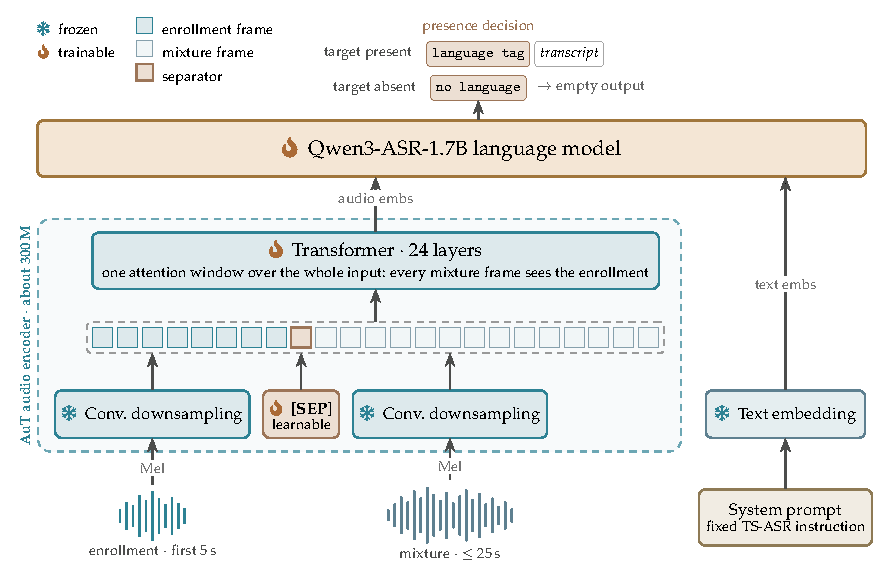
\includegraphics[width=\linewidth]{figures/input-construction.pdf}
  \caption{AmphionASR~2.0 in TS-ASR mode. The enrollment (first 5\,s) and the mixture (at most 25\,s) get separate Mel features and pass separately through the frozen convolutional downsampling of the AuT encoder. After the convolution, a learnable \septok vector joins them into one sequence before the 24 Transformer layers, whose attention covers the whole input. The fixed system prompt enters the language model through the frozen text embedding, and the language tag at the start of the output carries the present or absent decision.}
  \label{fig:input}
\end{figure}

\paragraph{Separate convolution.}
Each segment gets its own Mel features, is zero-padded to a whole number of Mel hops and passes through the convolutional downsampling of AuT on its own, with its own positional encoding.
The last enrollment frame and the first mixture frame therefore never share a convolutional receptive field.
The convolution layers stay frozen during fine-tuning.

\paragraph{A learnable separator.}
\septok is a trainable 1024-dimensional vector and is inserted only in TS-ASR mode; plain and hotword ASR neither split the input nor insert it.
The language model thus receives one audio token for each convolutional output of the enrollment and the mixture, plus one for \septok.

\paragraph{Global attention.}
The Qwen3-ASR encoder supports chunked attention windows of 1--8\,s~\cite{shi2026qwen3asr}.
With chunking, mixture frames far from the enrollment could not attend to it, so both training and inference use a single window that covers the whole input.
Every mixture frame can attend to the enrollment segment in every layer.

\paragraph{Empty output.}
When the target is present, the model outputs a language tag followed by the transcript; when the target is absent, the tag marks no language and the transcript is empty.
The presence decision is concentrated on this tag, so an application can set a more conservative threshold on its probability.

\subsection{Task formats}
\label{subsec:model_tasks}

The three tasks share all parameters and differ only in the system prompt and in the audio layout (\Cref{tab:tasks}).
A 5\,s enrollment is recommended, and 3\,s is also supported.
One request carries at most 30\,s of audio, so in TS-ASR mode the mixture is at most 30\,s minus the enrollment length; longer recordings must be segmented first.

\begin{table}[t]
  \caption{Input format of the three tasks.}
  \label{tab:tasks}
  \centering
  \small
  \begin{tabularx}{\linewidth}{@{}l>{\raggedright\arraybackslash}Xl@{}}
    \toprule
    Task & System prompt & Audio \\
    \midrule
    Plain ASR & empty & whole clip, $\le$ 30\,s \\
    Hotword ASR & list of hotwords & whole clip, $\le$ 30\,s \\
    TS-ASR & fixed instruction & enrollment (first 5\,s) + \septok + mixture ($\le$ 25\,s) \\
    \bottomrule
  \end{tabularx}
\end{table}

% Data. Sources: refs/docs/train_eval_data.md §1--5; HTML §4. Section layout (overview,
% corpus table, pipeline paragraphs) follows the data sections of the 1.0 report and
% Kimi-Audio, per AGENTS.md rule 6. Sampling weights, mixing probabilities and counterpart
% ratios are deliberately left out (user, 2026-10-31).

\section{Data}
\label{sec:data}

Training has two stages (\Cref{sec:training}).
Stage~1, multi-task supervised fine-tuning, uses plain ASR, hotword ASR, synthetic two- and three-talker target-speaker mixtures and turn-taking samples cut from meeting corpora.
This section describes the data of stage~2, target-speaker robustness training.
Target-speaker samples make up most of the stage-2 data: online mixtures, scene pools, turn-taking samples and real meeting windows, plus samples in which nobody speaks or a sentence is surrounded by babble.
The rest are plain and hotword ASR samples, intended to retain those capabilities.
\Cref{tab:corpora} lists the public corpora; the stage-2 data also include a small amount of domain-specific speech and meeting-room noise floors, which are not listed.

\begin{table}[t]
  \caption{Public corpora used in stage~2.}
  \label{tab:corpora}
  \centering
  \small
  \begin{tabularx}{\linewidth}{@{}>{\raggedright\arraybackslash}p{3.4cm}>{\raggedright\arraybackslash}X@{}}
    \toprule
    Use & Corpora \\
    \midrule
    Target-speaker voices & AISHELL-2~\cite{du2018aishell2}, LibriSpeech~\cite{panayotov2015librispeech}, KeSpeech~\cite{tang2021kespeech}, MagicData, Emilia~\cite{he2024emilia} \\
    Interferers and real conversations & AliMeeting~\cite{yu2022m2met}, AISHELL-4~\cite{fu2021aishell4}, MagicData-RAMC~\cite{yang2022open}, AMI~\cite{carletta2005ami}, CHiME-6~\cite{watanabe2020chime6}, Emilia conversations \\
    Plain ASR & WenetSpeech~\cite{zhang2022wenetspeech}, GigaSpeech~\cite{chen2021gigaspeech}, Common Voice~\cite{ardila2020common}, FLEURS, KeSpeech, AISHELL-2, LibriSpeech, 3D-Speaker~\cite{zheng2023speaker}, Voice-in-the-Wild-2M~\cite{xie2026megaasr} \\
    Noise & MUSAN~\cite{snyder2015musan}, WHAM!~\cite{wichern2019wham}, DNS Challenge noise~\cite{dubey2023icassp}, AudioSet, synthetic babble \\
    Room impulse responses & DNS Challenge, OpenSLR 26 and 28, MIT measured rooms~\cite{traer2016statistics} \\
    \bottomrule
  \end{tabularx}
\end{table}
% TODO: add citations for FLEURS, AudioSet and OpenSLR 26/28 (not yet in refs INDEX).

\subsection{Online mixing}
\label{subsec:data_mixing}

Most target-speaker samples are synthesized on the fly when they are loaded, so a source item yields a different mixture each time it is drawn.
A mixture has up to four interferers and varies in signal-to-interference ratio and overall level; speakers may pass through near-field or far-field room responses, and noise is added on top of a noise floor.
The enrollment is a random 1--20\,s crop and may be degraded by another voice, a low level, narrowband filtering, leading silence, telephone codecs or clipping.
The target may enter or leave midway.
For absent samples, the target is removed from the mixture and the transcript is empty.

\subsection{Scene pools and target-absent counterparts}
\label{subsec:data_scenes}

Random mixing does not reproduce structures that are common in meetings and conversations: two people taking turns, someone else picking up a sentence, the target saying only a word or two, or several people talking at once.
We build scene pools for these structures, following three principles.

\paragraph{Every scene type has target-absent counterparts.}
A counterpart keeps the same scene but enrolls another person, sometimes a similar-sounding one, and its reference transcript is empty.
During development, some scene types, such as turn-taking, were almost always target-present in training.
On those scenes the model still transcribed someone in about a quarter of samples after the enrollment was replaced by that of an unrelated person.
Adding counterparts to these scene types lowered the target-absent false-alarm rate from 4.9\% to 1.9\%, measured at the threshold that fixes the empty-output rate at 5\%.

\paragraph{More sources of target speakers.}
Besides AISHELL-2, Mandarin targets come from KeSpeech, in which the same speaker is recorded once in Mandarin and once in dialect, and from MagicData speakers.
Each new source covers all scene types.

\paragraph{The enrollment never contains the target sentence.}
In corpora where a speaker reads the same text several times, the enrollment could be the target sentence itself; such samples are excluded so that the target cannot be copied from the enrollment.

\subsection{Real meeting windows and label checks}
\label{subsec:data_real}

We cut real multi-talker windows from the training sets of AliMeeting, AISHELL-4, MagicData-RAMC and Emilia, and decide from the utterance-level timeline whether the enrolled speaker talks in each window.
Windows labeled ``enrolled speaker absent'' in which a check found the enrolled speaker talking are excluded.

\subsection{No speech and background babble}
\label{subsec:data_babble}

We add samples with only noise, music or babble and an empty target, intended to keep the model from producing text when nobody speaks.
We also add whole sentences with babble before, after and during them, intended to keep the model from dropping a sentence spoken inside babble.

% Training. Sources: refs/docs/train_eval_data.md §1, refs/docs/model_arch.md §4; HTML §5.

\section{Training}
\label{sec:training}

AmphionASR~2.0 starts from Qwen3-ASR-1.7B and is trained in two stages, both updating all parameters except the frozen ones listed in \Cref{tab:training}.
Stage~1 consists of three rounds of multi-task supervised fine-tuning.
Stage~2 continues from the stage-1 model with target-speaker robustness training in five segments.
Each segment starts from the weights of the previous one, and its data recipe is adjusted according to the evaluation of the previous segment.

\begin{table}[t]
  \caption{Training setup.}
  \label{tab:training}
  \centering
  \small
  \begin{tabularx}{\linewidth}{@{}>{\raggedright\arraybackslash}p{4.4cm}>{\raggedright\arraybackslash}X@{}}
    \toprule
    Item & Setting \\
    \midrule
    Initialization & Qwen3-ASR-1.7B~\cite{shi2026qwen3asr} \\
    Stage 1: multi-task supervised fine-tuning & Plain ASR, hotword ASR, synthetic target-speaker mixtures and meeting turn-taking data; three rounds \\
    Stage 2: target-speaker robustness training & Five segments continued from the stage-1 model \\
    Parameters updated & All, except the text embeddings and the convolution layers of the AuT encoder, which are frozen; \septok is trained \\
    Loss & Cross-entropy on the text positions to be predicted only \\
    Released weights & Parameter-wise average of the last three checkpoints~\cite{wortsman2022model} \\
    \bottomrule
  \end{tabularx}
\end{table}

\paragraph{Weight averaging.}
The present-or-absent decision of a single checkpoint fluctuates: between neighboring checkpoints, the share of target-present samples with an empty output can differ by 4 percentage points.
We therefore release the parameter-wise average of the last three checkpoints~\cite{wortsman2022model}.

% Experiments. Numbers: refs/internal/html-report/data.json (v12, asr, babble,
% qwen3_hotwords) and supp.json (bench, hwv3), identical to the published HTML §6.
% Headline numbers re-derived from the AmphionEval records (fact-check block).
% Organization follows the headline-table + condition-breakdown layout of the
% 1.0 report §5 and Seed-ASR, per AGENTS.md rule 6.

\section{Experiments}
\label{sec:experiments}

\subsection{Setup}
\label{subsec:exp_setup}

\paragraph{Test sets.}
\Cref{tab:testsets} lists the test sets.
TS-ASR is evaluated on \tsbench (\Cref{sec:benchmark}); the other capabilities are evaluated on public test sets and in-house test sets.

\paragraph{Normalization and metrics.}
Mandarin normalization and the three TS-ASR metrics are defined in \Cref{subsec:bench_metrics}.
English is scored by word after the Whisper English normalizer~\cite{radford2023robust}.

\paragraph{Inference.}
AmphionASR~2.0 is served with vLLM~\cite{kwon2023vllm}, with greedy decoding, at most 512 generated tokens and the first 5\,s of each enrollment.
Every test set is evaluated on all of its items.

\paragraph{Baselines.}
For TS-ASR we compare with Xiaomi-CocktailASR-1~\cite{zhang2026xiaomi} in both its standard and its chain-of-thought (CoT) mode.
Of the related systems in \Cref{tab:design}, it is the only external one that transcribes a single enrolled speaker in Mandarin and outputs nothing when that speaker is absent.
MT-LLM is trained on English and German, SpeakerLM transcribes every speaker of a conversation, and DiCoW takes diarization output instead of an enrollment.
The CocktailASR-1 report does not link released weights, so we use those published on Hugging Face as \texttt{Ease3/Xiaomi-CocktailASR-1}, with the transformers inference code that comes with them (bf16, greedy decoding).
CocktailASR-1 runs on the same audio, the same first 5\,s of enrollment and the same scoring as AmphionASR~2.0.
That report samples the reference speech at random lengths of 1--4\,s.
On an earlier version of our test set, a fixed 3\,s crop and such a random crop gave group CERs that differed by at most about 7 points and essentially the same target-absent false-alarm rates.
For plain ASR we compare with Qwen3-ASR-1.7B~\cite{shi2026qwen3asr}, MiMo-V2.5-ASR, Ming-3.0-asr-tiny, VibeVoice-ASR-7B and Dolphin-CN-Dialect; all baseline numbers are measured by us on the same data with the same scoring.
% TODO: add citations for MiMo-V2.5-ASR, Ming-3.0-asr-tiny, VibeVoice-ASR-7B and
% Dolphin-CN-Dialect (official model cards); none is in refs INDEX yet.

\begin{table}[t]
  \caption{Test sets used in this report.}
  \label{tab:testsets}
  \centering
  \small
  \begin{tabularx}{\linewidth}{@{}l>{\raggedright\arraybackslash}X>{\raggedright\arraybackslash}p{3.0cm}@{}}
    \toprule
    Capability & Test set & Metrics \\
    \midrule
    TS-ASR & \tsbench (\Cref{sec:benchmark}): 24{,}101 samples in 248 subsets; synthetic degraded enrollment, entry and exit, short segments, noise and far field; real AliMeeting, AISHELL-4 and MagicData-RAMC test windows and web conversations & CER, empty-output rate, false-alarm rate \\
    Babble robustness & In-house, 16 splits $\times$ 200 samples & false-alarm rate, CER, WER \\
    Hotword ASR & AISHELL-1 and Common Voice English hotword subsets (correct word plus 10 distractors); in-house retrieved-candidate test (264{,}681 requests) & CER, WER, hotword recall, false-alarm rate \\
    Plain ASR & AISHELL-1~\cite{bu2017aishell1}, AISHELL-2~\cite{du2018aishell2}, AISHELL-3~\cite{shi2021aishell3}, MagicData, THCHS-30~\cite{wang2015thchs30}, KeSpeech~\cite{tang2021kespeech}, Common Voice~\cite{ardila2020common}, WenetSpeech~\cite{zhang2022wenetspeech}, LibriSpeech~\cite{panayotov2015librispeech}, MLS~\cite{pratap2020mls}, GigaSpeech~\cite{chen2021gigaspeech}, TALCS~\cite{li2022talcs}, WenetSpeech-Chuan, CHiME-4~\cite{vincent2017analysis} & CER, WER \\
    \bottomrule
  \end{tabularx}
\end{table}

\subsection{Target-speaker recognition}
\label{subsec:exp_tsasr}

\Cref{tab:ts_overall} gives the overall results on \tsbench.
With the target present, AmphionASR~2.0 reaches 13.1\% CER, about two fifths of the 33.4\% of CocktailASR-1, at a similar empty-output rate (2.9\% and 2.7\%).
The largest gap is with the target absent: the false-alarm rates of AmphionASR~2.0 are 3.8\% on synthetic scenes and 2.6\% on real conversations, against 64.5\% and 96.1\% for CocktailASR-1.
With chain of thought enabled, CocktailASR-1 reaches 39.6\% CER on target-present samples and a 61.9\% false-alarm rate on target-absent samples.
These numbers compare whole systems: no controlled experiment in this report separates the contribution of the training data from that of the architecture or the model size.
The same team also built \tsbench and the training data of AmphionASR~2.0.
Training scene types such as turn-taking, hand-overs, short sentences and similar voices also appear in the benchmark, and the real part measures in-domain behavior for AmphionASR~2.0 because the training splits of its corpora are used in training (\Cref{sec:limitations}).

\begin{table}[t]
  \caption{Overall TS-ASR results on \tsbench (\%, lower is better). Bold marks the best value in each row.}
  \label{tab:ts_overall}
  \centering
  \small
  \begin{tabular}{@{}lccc@{}}
    \toprule
    Metric & AmphionASR 2.0 & CocktailASR-1 & CocktailASR-1 $\cdot$ CoT \\
    \midrule
    Target present $\cdot$ CER & \best{13.1} & 33.4 & 39.6 \\
    Target present $\cdot$ empty output & 2.9 & \best{2.7} & 3.0 \\
    Target absent $\cdot$ false alarm (all) & \best{3.7} & 67.8 & 61.9 \\
    \quad synthetic scenes & \best{3.8} & 64.5 & 58.8 \\
    \quad real meetings, calls and web conversations & \best{2.6} & 96.1 & 87.7 \\
    \midrule
    Real conversations $\cdot$ target-present CER & \best{9.2} & 30.8 & 27.2 \\
    Target alone, one 2--6\,s sentence $\cdot$ CER & 5.5 & 4.1 & \best{3.6} \\
    Four others speaking, target absent $\cdot$ false alarm & \best{8.3} & 89.2 & 77.5 \\
    Babble only $\cdot$ false alarm & \best{3.3} & 29.2 & 75.0 \\
    \bottomrule
  \end{tabular}
  \par\smallskip
  {\footnotesize 24{,}101 samples in 248 subsets (12{,}950 target-present, 11{,}151 target-absent); the first 5\,s of each enrollment recording are used. CER is pooled over all target-present samples; the empty-output and false-alarm rates are counted per sample.\par}
\end{table}

\begin{figure}[t]
  \centering
  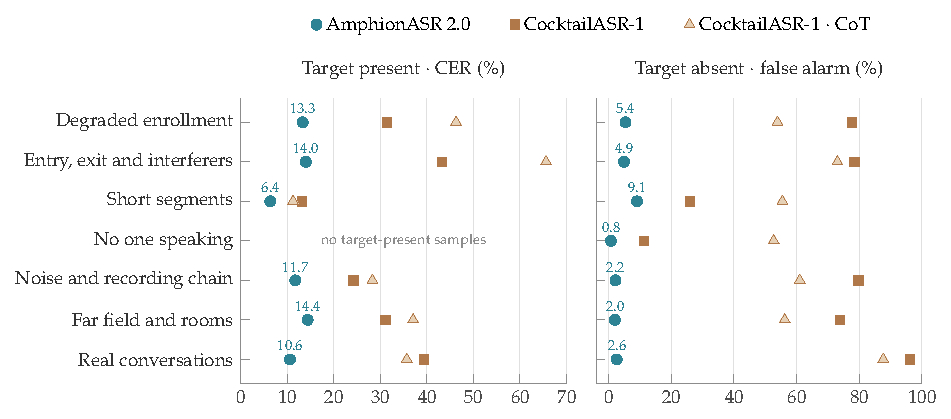
\includegraphics[width=\linewidth]{figures/section-results.pdf}
  \caption{Results pooled by section of \tsbench. Left: target-present CER; right: target-absent false-alarm rate. The ``no one speaking'' section has target-absent samples only. \Cref{app:scenarios} gives the results by scenario.}
  \label{fig:sections}
\end{figure}

By section (\Cref{fig:sections}), AmphionASR~2.0 has a lower target-present CER than CocktailASR-1 in every section, and a target-absent false-alarm rate more than an order of magnitude lower in every section except short segments.
The false alarms of CocktailASR-1 are concentrated in conditions where other people talk at length.
Its false-alarm rate is about 11\% when nobody speaks and 11.0\% on 1.2--6\,s segments with only others speaking, against 71.8--100\% in the target-absent groups of all other sections except short segments (\Cref{tab:scenarios}).
When the target alone says one short sentence, the two systems have similar CER (4.2\% and 4.8\%).

\subsection{How the evaluation conditions change the conclusion}
\label{subsec:exp_conditions}

\Cref{tab:conditions} regroups the subsets of \tsbench by whether common evaluations also cover them.
The first four rows are cases that common evaluations can measure: only the target speaking, nobody speaking, and the target mixed with one interferer.
With only the target speaking, all three systems stay at or below 7.5\% CER, and they are almost identical on real recordings; the CoT mode even has the lowest CER in the synthetic condition (3.8\%).
If an evaluation also includes target-absent samples in which nobody speaks, as the evaluation of AmphionASR~1.0 did, CocktailASR-1 has a false-alarm rate of 10.8\%, which looks acceptable.
The usual two-talker mixture does separate the target-present CERs (7.3\% and 21.3\%) but still misses the main difference.
With others talking and the target absent, CocktailASR-1 transcribes someone else on 85.8\% of synthetic and 96.1\% of real samples, against 3.5\% and 2.6\% for AmphionASR~2.0.
With the target present and 2--4 interferers, the CER of CocktailASR-1 rises to 65.7\%, against 18.9\% for AmphionASR~2.0.

\begin{table}[t]
  \caption{How the evaluation conditions change the conclusion (\%, lower is better). Bold marks the best value in each row.}
  \label{tab:conditions}
  \centering
  \small
  \begin{tabularx}{\linewidth}{@{}>{\raggedright\arraybackslash}Xrccc@{}}
    \toprule
    Condition & Samples & AmphionASR 2.0 & CocktailASR-1 & CoT \\
    \midrule
    \multicolumn{5}{@{}l}{\textit{Conditions that common evaluations also cover}} \\
    Only the target speaks $\cdot$ synthetic $\cdot$ CER & 540 & 4.6 & 5.5 & \best{3.8} \\
    Only the target speaks $\cdot$ real windows $\cdot$ CER & 194 & 7.5 & \best{7.3} & 7.5 \\
    Nobody speaks $\cdot$ false alarm & 720 & \best{0.1} & 10.8 & 58.1 \\
    Target + 1 interferer, target present $\cdot$ CER & 480 & \best{7.3} & 21.3 & 61.3 \\
    \midrule
    \multicolumn{5}{@{}l}{\textit{Conditions common in real use but not covered by common evaluations}} \\
    Target + 2--4 interferers, target present $\cdot$ CER & 1{,}080 & \best{18.9} & 65.7 & 86.5 \\
    Real windows with 3+ talkers, target present $\cdot$ CER & 126 & \best{18.1} & 64.7 & 40.3 \\
    Others speaking, target absent $\cdot$ synthetic $\cdot$ false alarm & 480 & \best{3.5} & 85.8 & 66.7 \\
    Others speaking, target absent $\cdot$ real recordings $\cdot$ false alarm & 1{,}191 & \best{2.6} & 96.1 & 87.7 \\
    A similar-sounding person speaking, target absent $\cdot$ false alarm & 540 & \best{18.0} & 73.9 & 89.3 \\
    \bottomrule
  \end{tabularx}
  \par\smallskip
  {\footnotesize Synthetic ``only the target speaks'': 3 subsets (a whole clip, one short phrase, one 2--6\,s sentence); ``target + 1 interferer'': 4 subsets (continuous speech, simultaneous start, interjection, about 1\,s of speech); ``target + 2--4 interferers'': 9 subsets; ``nobody speaks'': 6 subsets (noise, music, traffic, near silence, very short and long clips); synthetic ``others speaking'': 4 subsets (1, 2 and 4 interferers, long clips); ``similar-sounding person'': 3 subsets. Target-present rows on real windows use clean enrollments only; the real target-absent row covers all target-absent samples of the real-conversation section. CoT: CocktailASR-1 in chain-of-thought mode.\par}
\end{table}

\paragraph{Paired subsets locate weaknesses.}
Two groups of target-absent samples are paired: the mixture is identical item by item, and only the enrollment changes, to that of a random person or of someone who sounds like a speaker in the mixture.
With a random enrollment, false alarms from AmphionASR~2.0 are rare (0.0\% on 6--18\,s segments and 4.7\% on one short phrase); with a similar-sounding enrollment, the rates rise to 12.5\% and 22.7\%.
This is the main remaining weakness of AmphionASR~2.0 (\Cref{sec:limitations}), and an evaluation that enrolls only random people would not reveal it.

\paragraph{Synthetic conditions against real recordings.}
The same AliMeeting windows exist as near-field and far-field recordings, which lets us check the synthetic far-field conditions against real ones (\Cref{tab:nearfar}).
The two agree on enrollment--mixture mismatch: with a far-field enrollment and a near-field mixture, the empty-output rate of AmphionASR~2.0 rises from 2.5\% to 6.7\% on synthetic data and from 0.9\% to 5.2\% on real recordings.
The synthetic far-field mixture, however, is harsher than a real meeting room.
With a near-field enrollment, switching the mixture to far field raises CER from 8.6\% to 16.9\% on synthetic data but only from 4.5\% to 6.4\% on real recordings.
We therefore use the synthetic subsets to find which factors the model is sensitive to, and the real subsets to measure how large the effects are.

\begin{table}[t]
  \caption{Synthetic far-field conditions against real recordings (AmphionASR~2.0, target present, CER / empty output, \%).}
  \label{tab:nearfar}
  \centering
  \small
  \begin{tabular}{@{}lcc@{}}
    \toprule
    Enrollment $\cdot$ mixture & Synthetic & Real AliMeeting \\
    \midrule
    Near-field enrollment $\cdot$ near-field mixture (baseline) & 8.6 / 2.5 & 4.5 / 0.9 \\
    Near-field enrollment $\cdot$ far-field mixture & 16.9 / 1.7 & 6.4 / 1.7 \\
    Far-field enrollment $\cdot$ near-field mixture & 10.6 / 6.7 & 10.7 / 5.2 \\
    Far-field enrollment $\cdot$ far-field mixture & 20.6 / 3.3 & 6.8 / 0.9 \\
    \bottomrule
  \end{tabular}
  \par\smallskip
  {\footnotesize Synthetic: the same base scenes (target plus one or two interferers), far field from measured room responses, 120 samples per cell. Real: the same 115 AliMeeting test windows, clean enrollments only; near field is the speaker's headset microphone, the near-field mixture is the sum of all headsets (level-matched to the far-field mixture), and far field is the first array channel.\par}
\end{table}

\subsection{Real meetings, phone calls and web conversations}
\label{subsec:exp_real}

The windows in \Cref{tab:real} are taken directly from the test sets of public corpora.
The false-alarm rate per corpus is 1--5\% for AmphionASR~2.0 and 74--100\% for CocktailASR-1.
With the target present, CocktailASR-1 also has a higher CER, for example 38.2\% on AliMeeting against 6.8\% for AmphionASR~2.0.
When the enrollment clip contains another voice, the target-present CER of AmphionASR~2.0 is 6--11 points higher than with a clean enrollment, while its target-absent false-alarm rate does not rise.

\begin{table}[t]
  \caption{Real meetings, phone calls and web conversations (\%). Target-present rows give CER / empty output; target-absent rows give the false-alarm rate. Bold marks the best value in each row.}
  \label{tab:real}
  \centering
  \small
  \begin{tabularx}{\linewidth}{@{}>{\raggedright\arraybackslash}Xrccc@{}}
    \toprule
    Corpus and condition & Samples & AmphionASR 2.0 & CocktailASR-1 & CoT \\
    \midrule
    AliMeeting far-field meetings (present) & 115 & \best{6.8 / 0.9} & 38.2 / 0.0 & 36.9 / 0.0 \\
    AliMeeting far-field meetings (absent) & 100 & \best{1.0} & 100.0 & 97.0 \\
    AISHELL-4 far-field meetings (present) & 141 & \best{15.0 / 5.0} & 27.7 / 0.0 & 23.0 / 0.0 \\
    AISHELL-4 far-field meetings (absent) & 140 & \best{5.0} & 100.0 & 97.1 \\
    MagicData-RAMC phone calls (present) & 100 & \best{13.3 / 0.0} & 16.1 / 0.0 & 16.0 / 0.0 \\
    MagicData-RAMC phone calls (absent) & 100 & \best{5.0} & 96.0 & 83.0 \\
    Emilia web conversations, pseudo-labels (present) & 148 & \best{10.2 / 2.0} & 19.7 / 0.0 & 16.6 / 0.0 \\
    Emilia web conversations, pseudo-labels (absent) & 150 & \best{2.7} & 74.0 & 50.0 \\
    AliMeeting near/far-field pairs (present) & 460 & \best{7.1 / 2.2} & 36.3 / 0.0 & 31.5 / 0.2 \\
    AliMeeting near/far-field pairs (absent) & 400 & \best{2.0} & 99.8 & 90.5 \\
    \midrule
    Real meetings $\cdot$ enrollment contains another voice (present) & 62 & \best{15.6 / 1.6} & 60.8 / 0.0 & 64.1 / 0.0 \\
    Real meetings $\cdot$ enrollment contains another voice (absent) & 77 & \best{1.3} & 97.4 & 96.1 \\
    AliMeeting pairs $\cdot$ enrollment contains another voice (present) & 164 & \best{18.5 / 4.9} & 94.1 / 0.0 & 87.0 / 0.6 \\
    AliMeeting pairs $\cdot$ enrollment contains another voice (absent) & 224 & \best{2.2} & 100.0 & 96.9 \\
    \bottomrule
  \end{tabularx}
  \par\smallskip
  {\footnotesize Windows are cut directly from the human-annotated test sets of AliMeeting, AISHELL-4 and MagicData-RAMC and from Emilia web conversations, without mixing; Emilia references come from automatic diarization and recognition. ``Enrollment contains another voice'' means that another speaker talks for at least 0.3\,s within the first 5\,s of the enrollment clip.\par}
\end{table}

\subsection{Enrollment quality}
\label{subsec:exp_enrollment}

\Cref{tab:enrollment} changes only the enrollment on the same base scenes.
Another voice mixed into the enrollment has the largest effect, whereas leading silence, narrowband audio, a noise floor and reverberation change the results of AmphionASR~2.0 little.
With only 1\,s of speech in the enrollment, the target-absent false-alarm rate rises to 23.3\%.
During development we also swept the enrollment length: 3\,s and 5\,s both work, while 8\,s or more increases the empty-output rate with the target present; this observation has not been analyzed further.

\begin{table}[t]
  \caption{Effect of enrollment quality (\%). For each system: target-present CER, target-present empty-output rate and target-absent false-alarm rate.}
  \label{tab:enrollment}
  \centering
  \small
  \begin{tabular}{@{}lcccccc@{}}
    \toprule
    & \multicolumn{3}{c}{AmphionASR 2.0} & \multicolumn{3}{c}{CocktailASR-1} \\
    \cmidrule(lr){2-4}\cmidrule(l){5-7}
    Enrollment & CER & Empty & FA & CER & Empty & FA \\
    \midrule
    Clean enrollment & 11.9 & 2.7 & 0.7 & 20.9 & 0.7 & 74.0 \\
    Only 1\,s of speech (rest zero-padded) & 19.8 & 2.0 & 23.3 & 86.1 & 8.0 & 85.3 \\
    Leading silence & 11.4 & 0.7 & 2.0 & 22.4 & 0.0 & 76.7 \\
    4\,kHz narrowband & 10.2 & 1.3 & 2.0 & 25.2 & 1.3 & 74.7 \\
    Noise floor, 10\,dB SNR & 11.4 & 2.0 & 1.3 & 33.9 & 0.7 & 74.7 \\
    Reverberation & 10.6 & 1.3 & 2.0 & 24.4 & 2.0 & 72.0 \\
    Another voice mixed in, 10\,dB SIR & 16.2 & 2.7 & 8.0 & 24.5 & 0.0 & 78.7 \\
    Another voice mixed in, 0\,dB & 27.6 & 15.3 & 15.3 & 36.7 & 5.3 & 74.0 \\
    Very low level & 14.5 & 2.7 & 7.3 & 27.1 & 2.0 & 74.7 \\
    \bottomrule
  \end{tabular}
  \par\smallskip
  {\footnotesize The same base scenes (one or two interferers) with only the enrollment audio changed; 150 samples per cell.\par}
\end{table}

\subsection{Background babble}
\label{subsec:exp_babble}

\Cref{tab:babble} checks two behaviors in plain ASR mode: whether the model produces text when only babble is present, and whether it drops a sentence spoken inside babble.
With babble formed only from multi-talker read speech, the false-alarm rate of AmphionASR~2.0 is 0.5\%; with real crowd recordings it is 3.5\% (WHAM!) and 7.5\% (FSD50K).
Even at 5\,dB, the error rate on a whole sentence inside babble stays below 3.4\%, against 1.19\% CER and 1.83\% WER without babble.

\begin{table}[t]
  \caption{Robustness to background babble (AmphionASR~2.0, plain ASR mode, \%, 200 samples per condition).}
  \label{tab:babble}
  \centering
  \small
  \begin{tabular}{@{}lc@{\hspace{2.2em}}lc@{}}
    \toprule
    Babble only (false-alarm rate) & & One sentence inside babble & CER / WER \\
    \midrule
    Mandarin babble $\cdot$ far & 0.50 & Mandarin $\cdot$ no babble (control) & 1.19 \\
    Mandarin babble $\cdot$ mid & 0.50 & Mandarin $\cdot$ 20\,dB & 1.29 \\
    English babble $\cdot$ far & 0.50 & Mandarin $\cdot$ 10\,dB & 1.76 \\
    English babble $\cdot$ mid & 0.50 & Mandarin $\cdot$ 5\,dB & 3.33 \\
    Real ambient voices $\cdot$ WHAM! & 3.50 & Mandarin $\cdot$ 10\,dB, no leading or trailing gap & 1.90 \\
    Real crowd noise $\cdot$ FSD50K & 7.50 & English $\cdot$ no babble (control) & 1.83 \\
    & & English $\cdot$ 20\,dB & 1.77 \\
    & & English $\cdot$ 10\,dB & 2.22 \\
    & & English $\cdot$ 5\,dB & 3.38 \\
    & & English $\cdot$ 10\,dB, no leading or trailing gap & 2.09 \\
    \bottomrule
  \end{tabular}
  \par\smallskip
  {\footnotesize Babble is built from multi-talker read speech whose speakers do not overlap with the test speakers, and from real crowd recordings in WHAM!~\cite{wichern2019wham} and FSD50K~\cite{fonseca2022fsd50k}. Babble is present before, after and during the sentence unless stated otherwise; Mandarin is scored by CER and English by WER.\par}
\end{table}

\subsection{Hotword recognition}
\label{subsec:exp_hotwords}

\Cref{tab:hotwords_given} gives results when the candidate list holds the correct hotword and 10 random distractors.
Given the list, AmphionASR~2.0 recalls 98.2\% of the hotwords in English and 99.8\% in Mandarin, against 91.3\% and 96.0\% for Qwen3-ASR-1.7B.

\begin{table}[t]
  \caption{Hotwords with a list that holds the correct word and 10 random distractors (\%). Bold marks the best value in each row.}
  \label{tab:hotwords_given}
  \centering
  \small
  \begin{tabular}{@{}lcc@{}}
    \toprule
    Condition & AmphionASR 2.0 & Qwen3-ASR-1.7B \\
    \midrule
    \multicolumn{3}{@{}l}{\textit{AISHELL-1 hotword subset}} \\
    No hotwords $\cdot$ CER & \best{0.37} & 1.48 \\
    No hotwords $\cdot$ hotword recall & \best{98.5} & 85.0 \\
    With hotwords $\cdot$ CER & \best{0.32} & 1.18 \\
    With hotwords $\cdot$ hotword recall & \best{99.8} & 96.0 \\
    \midrule
    \multicolumn{3}{@{}l}{\textit{Common Voice English hotword subset}} \\
    No hotwords $\cdot$ WER & 8.15 & \best{7.33} \\
    No hotwords $\cdot$ hotword recall & 59.7 & \best{64.1} \\
    With hotwords $\cdot$ WER & \best{5.42} & 5.56 \\
    With hotwords $\cdot$ hotword recall & \best{98.2} & 91.3 \\
    \bottomrule
  \end{tabular}
  \par\smallskip
  {\footnotesize All items. The correct hotword is always in the list, so this test asks whether the model uses the list once it is given. Distractor false-alarm rate of AmphionASR~2.0: 0.065\% in English and 0.000\% in Mandarin.\par}
\end{table}

A setting closer to real use draws the candidate list from a lexicon by retrieval, so the list contains homophone and near-homophone distractors and may not contain the correct word at all (\Cref{tab:hotwords_retrieved}).
In English all three models have low false-alarm rates, at most 6.5\% when the list contains the correct word.
AmphionASR~2.0 has the highest recall on Common Voice English (97.2\%), but its false-alarm rate on GigaSpeech (6.5\%) is clearly higher than that of Qwen3-ASR-1.7B (0.2\%).
Mandarin is the clearest weakness in this evaluation.
With the correct word in the list, AmphionASR~2.0 has a higher false-alarm rate than Qwen3-ASR-1.7B on six of the seven Mandarin sets (real speech: 21.7\% and 9.6\%), and without the correct word the gap widens (real speech: 39.8\% and 17.7\%).
Its false-alarm rates are lower than those of Ming-3.0-asr-tiny on every Mandarin set.
Recall is mixed: AmphionASR~2.0 is slightly higher on AISHELL-2 and AISHELL-3, while Qwen3-ASR-1.7B is higher on ContextASR, real speech, Common Voice Mandarin and KeSpeech.
On AISHELL-3, real speech and AISHELL-2, giving a retrieved list that contains the correct word lowers the recall of AmphionASR~2.0 compared with giving no list (AISHELL-3: 87.9\% and 95.0\%).
On these sets, the near-homophone distractors replace some words that the model writes correctly without a list.
Taken together, \Cref{tab:hotwords_given,tab:hotwords_retrieved} show that AmphionASR~2.0 uses the candidates it is given but does not yet reliably reject wrong candidates that sound alike.

% Generated from the published HTML report (refs/internal/html-report/, table 16;
% data: supp.json["hwv3"]). Bold marks the best value in each row: highest recall,
% lowest false-alarm rate.
\begin{table}[!tbp]
  \caption{Hotwords with candidate lists from lexicon retrieval (\%). Bold marks the best value in each row.}
  \label{tab:hotwords_retrieved}
  \centering
  \small
  \begin{tabular}{@{}lccc@{}}
    \toprule
    Data set & AmphionASR 2.0 & Qwen3-ASR-1.7B & Ming-3.0-asr-tiny \\
    \midrule
    \multicolumn{4}{@{}l}{\textit{List contains the correct word $\cdot$ hotword recall \%}} \\
    AISHELL-1 named entities$^\dagger$ & \best{94.4} & 76.0 & 78.8 \\
    ContextASR Mandarin & 81.4 & \best{92.8} & 71.9 \\
    Real speech (SpeechIO + WenetSpeech) & 79.6 & \best{89.5} & 80.9 \\
    Common Voice Mandarin & 80.8 & \best{85.9} & 74.5 \\
    AISHELL-2 & \best{80.6} & 79.7 & 74.7 \\
    AISHELL-3 & \best{87.9} & 86.4 & 82.2 \\
    KeSpeech & 76.8 & \best{82.8} & 77.3 \\
    GigaSpeech & 83.8 & 80.3 & \best{88.0} \\
    LibriSpeech other & 91.2 & 87.6 & \best{93.9} \\
    Common Voice English & \best{97.2} & 83.9 & 90.8 \\
    \midrule
    \multicolumn{4}{@{}l}{\textit{List contains the correct word $\cdot$ distractor false-alarm rate \%}} \\
    AISHELL-1 named entities$^\dagger$ & \best{5.4} & 17.7 & 24.6 \\
    ContextASR Mandarin & 63.8 & \best{35.2} & 90.7 \\
    Real speech (SpeechIO + WenetSpeech) & 21.7 & \best{9.6} & 25.3 \\
    Common Voice Mandarin & 26.1 & \best{14.2} & 36.1 \\
    AISHELL-2 & 18.8 & \best{14.5} & 27.2 \\
    AISHELL-3 & 13.0 & \best{11.8} & 20.1 \\
    KeSpeech & 22.3 & \best{13.2} & 28.8 \\
    GigaSpeech & 6.5 & \best{0.2} & 2.7 \\
    LibriSpeech other & \best{0.1} & 0.1 & 0.9 \\
    Common Voice English & 1.1 & \best{0.8} & 1.6 \\
    \midrule
    \multicolumn{4}{@{}l}{\textit{List lacks the correct word $\cdot$ false-alarm rate \%}} \\
    AISHELL-1 named entities$^\dagger$ & \best{15.7} & 27.5 & 47.4 \\
    ContextASR Mandarin & 85.2 & \best{63.9} & 99.2 \\
    Real speech (SpeechIO + WenetSpeech) & 39.8 & \best{17.7} & 52.7 \\
    Common Voice Mandarin & 52.9 & \best{25.4} & 66.7 \\
    AISHELL-2 & 40.3 & \best{20.8} & 53.5 \\
    AISHELL-3 & 32.3 & \best{21.1} & 48.1 \\
    KeSpeech & 43.4 & \best{23.4} & 59.5 \\
    GigaSpeech & 1.4 & \best{0.0} & 3.8 \\
    LibriSpeech other & 0.4 & \best{0.1} & 1.7 \\
    Common Voice English & 6.4 & \best{1.4} & 3.0 \\
    \midrule
    \multicolumn{4}{@{}l}{\textit{No list $\cdot$ hotword recall \%}} \\
    AISHELL-1 named entities$^\dagger$ & \best{97.4} & 68.2 & 81.8 \\
    ContextASR Mandarin & 81.5 & \best{89.1} & 48.3 \\
    Real speech (SpeechIO + WenetSpeech) & 83.2 & \best{85.4} & 81.9 \\
    Common Voice Mandarin & \best{77.1} & 75.0 & 76.6 \\
    AISHELL-2 & 82.5 & 78.6 & \best{84.7} \\
    AISHELL-3 & \best{95.0} & 83.1 & 91.9 \\
    KeSpeech & 73.7 & 72.5 & \best{82.2} \\
    GigaSpeech & 71.7 & 74.6 & \best{77.6} \\
    LibriSpeech other & 84.0 & 83.9 & \best{89.9} \\
    Common Voice English & 59.3 & 63.4 & \best{67.4} \\
    \bottomrule
  \end{tabular}
  \par\smallskip
  {\footnotesize All items, 264{,}681 requests in total, plain ASR mode. Mandarin lists hold 50 words retrieved from a pool of about 10{,}000 hotwords; English lists hold 50 (GigaSpeech, Common Voice) or 100 (LibriSpeech) words. All lists include homophone and near-homophone distractors; in the ``lacks the correct word'' condition every candidate is a distractor. Recall is counted over correct hotwords; the false-alarm rate is the share of utterances whose output contains some distractor more often than the reference does. Recall in the ``no list'' group is the share of the same hotwords written correctly without any hint. Real speech comes from SpeechIO and WenetSpeech test\_net and test\_meeting, with hotwords extracted and checked by a large language model. $^\dagger$Most AISHELL-1 test sentences appear in AISHELL-2, which AmphionASR~2.0 is trained on; this row is optimistic.\par}
\end{table}


\subsection{General recognition}
\label{subsec:exp_general}

We use public test sets to check whether adding TS-ASR has degraded plain ASR (\Cref{tab:asr_general}, plain ASR mode).
On the category means, AmphionASR~2.0 and Qwen3-ASR-1.7B obtain 3.39\% and 3.26\% on Mandarin (excluding AISHELL-1), 5.70\% and 5.14\% on English, and 9.11\% and 8.07\% on dialects and accents.
AmphionASR~2.0 is better on AISHELL-2, AISHELL-3 and MagicData and worse on WenetSpeech, WenetSpeech-Chuan and the KeSpeech dialects.
On WenetSpeech test\_net, about 30\% of the gap comes from differences in writing conventions (filler words, erhua, number formats and English words written in Chinese characters); the rest is a regression relative to the initialization.
% TODO: verify the 30% decomposition; the number comes from the published HTML §6.8
% and no computation for it was found in refs/docs or refs/internal.
Among the compared models, Ming-3.0-asr-tiny has the best means on Mandarin, English and dialects.
On the real noisy far-field English test set CHiME-4 et05\_real~\cite{vincent2017analysis}, AmphionASR~2.0 reaches 7.17\% WER.
These results check that plain recognition is retained; they do not show a lead in general recognition.

% Generated from the published HTML report (refs/internal/html-report/, table 17;
% data: data.json["asr"]). Bold marks the best value in each row.
\begin{table}[!tbp]
  \caption{Plain ASR on public test sets (CER / WER, \%). Bold marks the best value in each row.}
  \label{tab:asr_general}
  \centering
  \small
  \setlength{\tabcolsep}{4pt}
  \begin{tabular}{@{}lcccccc@{}}
    \toprule
    Test set & \begin{tabular}[b]{@{}c@{}}AmphionASR\\2.0\end{tabular} & \begin{tabular}[b]{@{}c@{}}Qwen3-ASR\\1.7B\end{tabular} & \begin{tabular}[b]{@{}c@{}}MiMo-V2.5\\ASR\end{tabular} & \begin{tabular}[b]{@{}c@{}}Ming-3.0\\asr-tiny\end{tabular} & \begin{tabular}[b]{@{}c@{}}VibeVoice\\ASR-7B\end{tabular} & \begin{tabular}[b]{@{}c@{}}Dolphin\\CN-Dialect\end{tabular} \\
    \midrule
    \multicolumn{7}{@{}l}{\textit{Mandarin}} \\
    WenetSpeech $\cdot$ test\_net & 5.49 & \best{4.49} & 4.87 & 5.06 & 17.62 & 6.64 \\
    WenetSpeech $\cdot$ test\_meeting & 5.51 & \best{4.69} & 5.28 & 4.91 & 20.89 & 6.58 \\
    AISHELL-1$^\dagger$ & \best{0.38} & 1.48 & 0.98 & 1.04 & 5.01 & 1.21 \\
    AISHELL-2 & 2.53 & 2.56 & 2.38 & \best{2.17} & 5.25 & 2.85 \\
    AISHELL-3 & \best{0.76} & 1.91 & 1.66 & 1.08 & 4.50 & 1.96 \\
    MagicData & 1.66 & 2.15 & 2.19 & \best{1.59} & 9.24 & 2.92 \\
    THCHS-30 & 3.81 & 2.85 & \best{1.38} & 2.80 & 6.36 & 4.12 \\
    KeSpeech $\cdot$ Mandarin & 2.32 & 2.37 & 2.38 & \best{1.76} & 11.89 & 2.46 \\
    Common Voice $\cdot$ Mandarin & 5.02 & 5.03 & 4.88 & \best{4.81} & 30.56 & 7.53 \\
    \cmidrule(l){2-7}
    Mandarin $\cdot$ mean & 3.39 & 3.26 & 3.13 & \best{3.02} & 13.29 & 4.38 \\
    \midrule
    \multicolumn{7}{@{}l}{\textit{English}} \\
    LibriSpeech $\cdot$ test-clean & 1.69 & 1.63 & 1.46 & \best{1.16} & 2.02 & 54.12 \\
    LibriSpeech $\cdot$ test-other & 3.65 & 3.37 & 3.45 & \best{2.39} & 5.52 & 63.74 \\
    MLS $\cdot$ English & 5.91 & 4.65 & 4.87 & \best{3.29} & 6.59 & 58.93 \\
    GigaSpeech & 9.09 & 8.70 & 8.82 & \best{8.38} & 9.65 & 62.23 \\
    Common Voice $\cdot$ English & 8.17 & 7.36 & 9.42 & \best{6.86} & 22.46 & 71.89 \\
    \cmidrule(l){2-7}
    English $\cdot$ mean & 5.70 & 5.14 & 5.61 & \best{4.42} & 9.25 & 62.18 \\
    \midrule
    \multicolumn{7}{@{}l}{\textit{Mandarin--English code-switching}} \\
    TALCS & 7.85 & 7.48 & 6.39 & \best{5.51} & 13.32 & 11.66 \\
    \midrule
    \multicolumn{7}{@{}l}{\textit{Dialects and accents}} \\
    KeSpeech $\cdot$ Beijing & 5.31 & 5.20 & 9.75 & \best{4.33} & 42.55 & 5.81 \\
    KeSpeech $\cdot$ Northeastern & 5.99 & 5.59 & 5.00 & \best{3.88} & 20.80 & 4.96 \\
    KeSpeech $\cdot$ Ji-Lu & 5.98 & 5.83 & 8.65 & \best{4.72} & 39.06 & 5.46 \\
    KeSpeech $\cdot$ Jiao-Liao & 6.42 & 6.43 & 9.47 & \best{4.90} & 45.92 & 5.59 \\
    KeSpeech $\cdot$ Zhongyuan & 4.64 & 4.30 & 7.62 & \best{3.23} & 36.81 & 3.96 \\
    KeSpeech $\cdot$ Lan-Yin & 5.99 & 5.90 & 11.21 & \best{4.98} & 51.00 & 5.77 \\
    KeSpeech $\cdot$ Jiang-Huai & 9.16 & 8.84 & 16.00 & \best{6.63} & 57.29 & 7.70 \\
    KeSpeech $\cdot$ Southwestern & 5.78 & 5.03 & 7.15 & \best{3.84} & 45.16 & 5.02 \\
    WenetSpeech-Chuan $\cdot$ easy & 14.66 & 11.77 & \best{11.69} & 13.92 & 58.92 & 13.03 \\
    WenetSpeech-Chuan $\cdot$ hard & 27.21 & \best{21.83} & 23.48 & 24.55 & 104.66 & 24.05 \\
    \cmidrule(l){2-7}
    Dialects and accents $\cdot$ mean & 9.11 & 8.07 & 11.00 & \best{7.50} & 50.22 & 8.13 \\
    \bottomrule
  \end{tabular}
  \par\smallskip
  {\footnotesize Plain ASR mode on every item of each test set; Chinese is scored by character and English by word. All models are scored on the same audio with the same text normalization. $^\dagger$Most AISHELL-1 test sentences also appear in the AISHELL-2 training set, which AmphionASR~2.0 uses; this row is optimistic and is excluded from the means.\par}
\end{table}



% Related work and comparisons. Sources: HTML §7; refs/docs/model_arch.md §6
% (design comparison); AmphionASR 1.0 PDF §3.5, §5.4; the papers of MT-LLM, SpeakerLM, DiCoW,
% TS-SUPERB, M2MeT 2.0, NOTSOFAR-1, Personal VAD, TST-Bench and the two ISCA TSE papers
% (refs/notes/papers/INDEX.yaml, added 2026-11-01). The CocktailASR-1 protocol
% note (refs/docs/plan.md §8) lives in the experimental setup.
% Placed after the experiments, as in the HTML and refs/docs/plan.md §5.

\section{Related Work and Comparisons}
\label{sec:related}

\paragraph{Evaluation.}
Common evaluations for speech separation and TSE are synthesized from read speech: WSJ0-2mix~\cite{hershey2016deep}, Libri2Mix~\cite{cosentino2020librimix}, and WHAM!~\cite{wichern2019wham} and WHAMR!~\cite{maciejewski2020whamr}, which add noise and reverberation to WSJ0-2mix.
TSE usually enrolls another utterance of the same speaker and reports signal-to-distortion ratios on mixtures in which the target is present~\cite{zmolikova2019speakerbeam, zmolikova2023neural}.
Multi-talker and target-speaker recognition often use LibriSpeechMix~\cite{kanda2020serialized}, synthesized from LibriSpeech.
Real meeting corpora such as AMI~\cite{carletta2005ami}, AISHELL-4~\cite{fu2021aishell4}, AliMeeting~\cite{yu2022m2met} and CHiME-6~\cite{watanabe2020chime6} are mainly used for diarization and multi-talker transcription and do not themselves define enrollments or target-absent samples.
Neither do the speaker-attributed ASR benchmark of M2MeT~2.0~\cite{liang2023second} or the far-field office meetings of NOTSOFAR-1~\cite{vinnikov2024notsofar}.
TS-SUPERB~\cite{peng2025tssuperb} conditions TS-ASR on an embedding of the enrollment but evaluates it on Libri2Mix.
An absent target has mainly been studied outside recognition.
Personal VAD~\cite{ding2020personal} labels each frame as non-speech, target-speaker speech or non-target speech.
Speaker extraction has been trained and evaluated with the target present or absent in mixtures of one and two talkers~\cite{borsdorf2021universal, zhang2023speaker}, and Delcroix et al.~\cite{delcroix2022listen} studied false extractions in TSE when the target is silent.
TST-Bench~\cite{lee2026who} asks a system to tag enrolled speakers and reject unknown ones in long synthetic conversations.
In \tsbench, target-absent samples make up nearly half of the benchmark, and enrollments and absent samples are also defined on real meeting and call recordings.

\paragraph{Models.}
Early TS-ASR work added speaker conditioning to encoder--decoder recognizers such as Whisper~\cite{radford2023robust}: prompt tuning~\cite{ma2023extending}, learnable speaker queries that extract prompts from the enrollment~\cite{guo2024sqwhisper}, or frame-level diarization outputs that modulate the encoder~\cite{polok2024target}.
DiCoW~\cite{polok2024dicow} develops the last into masks of silence, target, non-target and overlapping speech and needs no enrollment.
Among SpeechLLMs, MT-LLM~\cite{meng2024large} follows multi-talker instructions, one of which places a 3\,s clip of the target talker and 3\,s of silence before the mixture.
SpeakerLM~\cite{yin2025speakerlm} jointly diarizes and transcribes a conversation, attributing speech to registered speakers through their speaker embeddings and leaving out registered speakers who do not speak.
AmphionASR~1.0~\cite{amphion2026amphionasr} encodes the enrollment and the mixture separately and feeds them to the language model in sequence.
Xiaomi-CocktailASR-1~\cite{zhang2026xiaomi} and its precursor~\cite{zhang2025thinking} concatenate reference speech with the mixture into one input to the audio encoder and support an empty output when the target is absent as well as chain-of-thought reasoning.
Like CocktailASR-1, AmphionASR~2.0 lets the enrollment interact with the mixture inside the audio encoder, but it joins the two segments after the convolutional downsampling rather than on the waveform (\Cref{sec:model}).
\Cref{tab:design} summarizes these systems.

\begin{table}[!tbp]
  \caption{Speaker-conditioned recognizers related to AmphionASR~2.0.}
  \label{tab:design}
  \centering
  \footnotesize
  \setlength{\tabcolsep}{4pt}
  \begin{tabularx}{\linewidth}{@{}>{\raggedright\arraybackslash}p{2.2cm}>{\raggedright\arraybackslash}p{2.25cm}>{\raggedright\arraybackslash}X>{\raggedright\arraybackslash}p{2.3cm}>{\raggedright\arraybackslash}p{2.6cm}@{}}
    \toprule
    System & Model & How the target is specified & Absent target & TS-ASR evaluation \\
    \midrule
    AmphionASR 2.0 & About 1.7\,B: AuT encoder + Qwen3-1.7B & Enrollment audio (first 5\,s; random 1--20\,s in training), joined to the mixture by a learnable \septok after the encoder's convolution & Empty output; scored on paired absent samples & \tsbench: Mandarin, synthetic and real \\
    \addlinespace[2pt]
    AmphionASR 1.0~\cite{amphion2026amphionasr} & About 1.7\,B, plus a 2.6\,M hotword-retrieval adapter & Enrollment audio (3--5\,s) and mixture pass through the same encoder and enter the language model as two ordered spans & Empty output; 164 samples in which nobody speaks & In-house synthetic set \\
    \addlinespace[2pt]
    CocktailASR-1 \cite{zhang2026xiaomi} & About 8.9\,B: Data2Vec2 encoder~\cite{baevski2023efficient} + Qwen3-8B & Reference speech (random 1--4\,s), 1\,s of silence and the mixture, concatenated on the waveform & Empty output; separate absent test sets & LibriMix, LibriSpeechMix, AMI, AliMeeting \\
    \addlinespace[2pt]
    MT-LLM~\cite{meng2024large} & Llama-2-7B-chat with LoRA; Whisper and WavLM encoders & A 3\,s clip of the target and 3\,s of silence before the mixture, with an instruction & Not discussed & LibriSpeechMix; English and German \\
    \addlinespace[2pt]
    SpeakerLM~\cite{yin2025speakerlm} & Qwen2.5-7B-Instruct; SenseVoice-large encoder & Registered speakers: an embedding averaged over 2--10\,s clips, with the speaker's name & Registered speakers who do not speak are left out & Speaker-attributed transcription of AliMeeting, AISHELL-4, AISHELL-5 \\
    \addlinespace[2pt]
    DiCoW~\cite{polok2024dicow} & Whisper large-v3-turbo & No enrollment: frame-level masks from a diarization system & Not discussed & AMI, NOTSOFAR-1, Libri2Mix, LibriCSS \\
    \bottomrule
  \end{tabularx}
\end{table}

\subsection{Comparison with AmphionASR 1.0}
\label{subsec:related_v1}

\paragraph{Target-speaker recognition.}
On its in-house synthetic test set, AmphionASR~1.0 reports a target-present WER of 13.02\%, a miss rate of 4.13\% and a 6.10\% false-alarm rate on 164 target-absent samples in which nobody speaks~\cite{amphion2026amphionasr}.
That test set differs from \tsbench, so the numbers are not directly comparable.
The closest part of \tsbench is the ``no one speaking'' section, where the false-alarm rate of AmphionASR~2.0 is 0.8\%; \Cref{subsec:exp_conditions} shows what an evaluation restricted to target-present and silent samples misses.

\paragraph{General recognition.}
The two reports share 10 public test sets (\Cref{tab:vs_v1}).
Because their Mandarin normalizations differ, the table compares each version with the same reference model, Qwen3-ASR-1.7B, as measured in each report.
In English, 1.0 matches or slightly beats Qwen3-ASR-1.7B on LibriSpeech and trails it by 0.6--0.9 points on GigaSpeech and Common Voice, while 2.0 trails slightly on LibriSpeech, by less on GigaSpeech (0.40) and by 0.81 on Common Voice.
In Mandarin, the gap of 2.0 to Qwen3-ASR-1.7B is smaller than that of 1.0 on KeSpeech and Common Voice, and both versions are slightly better than Qwen3-ASR-1.7B on AISHELL-2.
On the two WenetSpeech subsets the gap of 2.0 is larger (1.01 points on test\_net, against 0.13 for 1.0).

\begin{table}[!tbp]
  \caption{Comparison with AmphionASR~1.0 on shared public test sets (CER / WER, \%). Each version is compared with Qwen3-ASR-1.7B as measured in its own report; negative differences mean better than Qwen3-ASR-1.7B.}
  \label{tab:vs_v1}
  \centering
  \small
  \setlength{\tabcolsep}{5pt}
  \begin{tabular}{@{}lcccccc@{}}
    \toprule
    & \multicolumn{3}{c}{AmphionASR 1.0 report~\cite{amphion2026amphionasr}} & \multicolumn{3}{c}{This report} \\
    \cmidrule(lr){2-4}\cmidrule(l){5-7}
    Test set & 1.0 & Qwen3-ASR & $\Delta$ & 2.0 & Qwen3-ASR & $\Delta$ \\
    \midrule
    LibriSpeech $\cdot$ test-clean & 1.59 & 1.61 & $-$0.02 & 1.69 & 1.63 & +0.06 \\
    LibriSpeech $\cdot$ test-other & 3.35 & 3.39 & $-$0.04 & 3.65 & 3.37 & +0.27 \\
    GigaSpeech & 9.53 & 8.68 & +0.85 & 9.09 & 8.70 & +0.40 \\
    Common Voice $\cdot$ English & 7.87 & 7.24 & +0.63 & 8.17 & 7.36 & +0.81 \\
    AISHELL-1$^\dagger$ & 1.34 & 1.58 & $-$0.24 & 0.38 & 1.48 & $-$1.10 \\
    AISHELL-2 & 2.65 & 2.77 & $-$0.12 & 2.53 & 2.56 & $-$0.04 \\
    KeSpeech (all dialects pooled) & 5.71 & 5.21 & +0.50 & 5.19 & 4.97 & +0.22 \\
    Common Voice $\cdot$ Mandarin & 5.21 & 5.06 & +0.15 & 5.02 & 5.03 & $-$0.01 \\
    WenetSpeech $\cdot$ test\_net & 5.17 & 5.04 & +0.13 & 5.49 & 4.49 & +1.01 \\
    WenetSpeech $\cdot$ test\_meeting & 6.30 & 5.85 & +0.45 & 5.51 & 4.69 & +0.82 \\
    \bottomrule
  \end{tabular}
  \par\smallskip
  {\footnotesize Both reports normalize English with the Whisper English normalizer but normalize Mandarin differently: the 1.0 report removes punctuation, unifies full- and half-width characters and converts Arabic numerals to Chinese characters, and this report additionally removes filler words and unifies erhua. Absolute Mandarin numbers are therefore not comparable across the two reports. $^\dagger$AISHELL-1 shares text with AISHELL-2, which 2.0 is trained on; the 2.0 entry in this row is optimistic.\par}
\end{table}

\FloatBarrier

% Limitations. Sources: HTML §8; refs/docs/ts_benchmark.md §6; refs/docs/plan.md §8;
% supp.json["ctx"] (context correction: 6.5% / 7.3%, 93.6%).

\section{Limitations}
\label{sec:limitations}

\paragraph{False alarms with many talkers or short sentences.}
With four other people speaking and the target absent, the false-alarm rate of AmphionASR~2.0 is 8.3\%; when a similar-sounding person says one short sentence and the target is absent, it is 22.7\%.

\paragraph{An empty output is not speaker verification.}
With a very poor enrollment or a very low SNR, a target-present sample may still yield an empty output, and a target-absent sample may still yield a false alarm.
Applications that need strict identity checks should add a speaker-verification step.

\paragraph{Regression in general recognition.}
AmphionASR~2.0 remains behind the model it was initialized from, Qwen3-ASR-1.7B, on WenetSpeech, WenetSpeech-Chuan, the KeSpeech dialects and English (\Cref{subsec:exp_general}).

\paragraph{Contextual correction.}
An in-house contextual-correction test has a speaker clarify an earlier word in the same utterance, for example by spelling out which character of a name is meant.
AmphionASR~2.0 rewrites the earlier mention according to the clarification only 6.5\% of the time (Qwen3-ASR-1.7B: 7.3\%), although 93.6\% of the clarifications themselves are transcribed correctly.
In TS-ASR mode, when the voice in the mixture is a text-to-speech clone of a person and the enrollment is that person's real recording, 11.6\% of samples produce an empty output.
% TODO: verify the 11.6% TTS-clone figure; it comes from the published HTML §8
% and was not found in supp.json["ctx"].

\paragraph{Near-homophone distractors in hotword lists.}
When the candidate list comes from lexicon retrieval and contains homophones and near-homophones, AmphionASR~2.0 writes wrong candidates into Mandarin output.
On real speech, its false-alarm rate is 21.7\% with the correct word in the list and 39.8\% without it, roughly twice that of Qwen3-ASR-1.7B in both cases (\Cref{subsec:exp_hotwords}).
In practice, the list should be kept short, with few near-homophones.

\paragraph{Punctuation and length.}
About 29\% of plain-ASR outputs carry punctuation, so post-processing is needed to punctuate the rest.
% TODO: verify the 29% punctuation share; it comes from the published HTML §8.
One request carries at most 30\,s of audio, and longer recordings must be segmented first.

\paragraph{Benchmark coverage.}
\tsbench is Mandarin only.
Its synthetic part uses read speech, without the prosody and interruptions of real conversation, and although its noise floors and room responses are partly real recordings, the mixing is synthetic.
The real part covers only meetings, phone calls and web conversations, with no in-car, outdoor or on-device recordings, and has only 100--460 samples per corpus.
References for the web conversations come from automatic diarization and recognition and contain some errors.
The training splits of the real meeting corpora, with different recordings and speakers, are used in training, so the real part measures in-domain behavior.
AISHELL-1 test text overlaps with AISHELL-2, which is used in training, and MagicData-RAMC assigns several speaker IDs to one person in some cases, so the real-call subset may contain training speakers.

% Conclusion. Source: HTML §9; synthesis only (paper-writing.mdc §6).

\section{Conclusion}
\label{sec:conclusion}

This report addressed target-speaker recognition in recordings where the enrolled speaker may or may not talk.
We proposed \tsbench, which will be released publicly.
Every condition is paired with target-present and target-absent samples.
The synthetic part is designed from errors observed in real use and changes one factor at a time, and the real part comes from the test sets of public meeting and call corpora and from web conversations.
With \tsbench, we showed that evaluations limited to a single talker, to samples with the target present or to silence can rate two systems as roughly equal.
Yet when others talk in real recordings, one of those systems almost always produces false alarms and the other rarely does.
We also presented AmphionASR~2.0, which joins the enrollment and the mixture with a learnable separator after the convolutional downsampling of its audio encoder and whose training data give every scene type target-absent counterparts.
Compared on \tsbench with Xiaomi-CocktailASR-1, a model about five times larger, AmphionASR~2.0 has a lower CER with the target present and a false-alarm rate more than an order of magnitude lower when others talk and the target is absent.
The difference holds on real meetings and calls.
The same weights also handle plain and hotword ASR, with a small regression in general recognition relative to the initial model.
False alarms when a similar-sounding person speaks briefly, near-homophone distractors in hotword lists, and this regression remain the main open problems.


% --- Bibliography: report-local cites + venue strings shipped with the template.
\bibliographystyle{template/IEEEtran2}
\setcitestyle{numbers}
\bibliography{template/venues, references}

\appendix
% Appendix. Sources: refs/docs/ts_benchmark.md §3 (synthesis rules);
% HTML appendix A (results by scenario, tables/scenarios.tex).

\section{Synthesis of the AmphionTS-Bench synthetic part}
\label{app:synthesis}

\paragraph{Levels.}
Each utterance is first normalized to $-25$\,dBFS and then scaled according to the signal-to-interference ratio of the condition, with an additional $\pm2$\,dB per interferer; the final mixture is peak-normalized to 0.5.

\paragraph{Timing.}
The target speaks only complete sentences.
The last sentence of an interferer may be cut off at the end of the clip, with a 30\,ms fade-out, to approximate segments cut by voice activity detection.

\paragraph{Noise floors and rooms.}
Noise floors come from WHAM!~\cite{wichern2019wham} (real ambient noise such as cafés, restaurants and streets), stationary AudioSet and Freesound excerpts distributed with the DNS Challenge~\cite{dubey2023icassp}, and white and pink noise, at $-65$ to $-35$\,dBFS.
Room responses come from measured responses in OpenSLR 28, simulated small, medium and large rooms, and the simulated responses of the DNS Challenge.

\paragraph{Background sounds.}
Background conditions use MUSAN~\cite{snyder2015musan} noise and music, AudioSet traffic, FSD50K~\cite{fonseca2022fsd50k} environmental events and crowds, synthetic babble from 5--20 test-split speakers, and Mandarin pop songs with accompaniment from MIR-1K, used only for evaluation.
% TODO: add citations for MIR-1K, AudioSet and OpenSLR 28 (not yet in refs INDEX).

\paragraph{Diagnostic conditions.}
Twelve subsets outside the sections cover 0\,dB enrollment contamination, clipping, 3.4\,kHz narrowband audio, $\mu$-law coding, and stacked outdoor and office conditions.

\section{Results by scenario}
\label{app:scenarios}

\Cref{tab:scenarios} lists the complete results on \tsbench grouped by scenario.
Each synthetic group changes a single condition on the same base scenes.

{\small
% Generated from the published HTML report (refs/internal/html-report/, table 20;
% data: data.json["v12"]["groups"]). Bold marks the best value in each row.
\begin{longtable}{@{}>{\raggedright\arraybackslash}p{5.4cm}crccc@{}}
  \caption{TS-ASR results on \tsbench by scenario (\%). Target-present rows give CER / empty output; target-absent rows give the false-alarm rate. Bold marks the best value in each row.}
  \label{tab:scenarios}\\
  \toprule
  Scenario & Target & Samples & AmphionASR 2.0 & CocktailASR-1 & CoT \\
  \midrule
  \endfirsthead
  \toprule
  Scenario & Target & Samples & AmphionASR 2.0 & CocktailASR-1 & CoT \\
  \midrule
  \endhead
  \bottomrule
  \endfoot
  \multicolumn{6}{@{}l}{\textit{Degraded enrollment}} \\
  Target present (degraded enrollment) & present & 1,200 & \best{13.3 / 1.9} & 33.1 / 1.8 & 51.7 / 6.0 \\
  Target absent (degraded enrollment) & absent & 1,200 & \best{5.8} & 76.3 & 50.2 \\
  Only 2--4 s of enrollment recorded (target present) & present & 450 & \best{13.5 / 1.8} & 26.9 / 0.2 & 31.8 / 1.1 \\
  Only 2--4 s of enrollment recorded (target absent) & absent & 450 & \best{4.2} & 81.1 & 63.8 \\
  \midrule
  \multicolumn{6}{@{}l}{\textit{Entry, exit and number of interferers}} \\
  Target present (entry, exit, number of interferers) & present & 1,920 & \best{15.1 / 3.0} & 46.8 / 4.3 & 68.5 / 7.5 \\
  Target absent (others speaking) & absent & 960 & \best{4.9} & 78.4 & 73.0 \\
  Target finishes, another speaker follows (no overlap) & present & 360 & \best{3.8 / 3.3} & 10.7 / 0.0 & 38.6 / 1.1 \\
  \midrule
  \multicolumn{6}{@{}l}{\textit{Short segments}} \\
  Target absent $\cdot$ 1.2--6 s segment (others speaking) & absent & 480 & \best{3.3} & 11.0 & 37.5 \\
  Target absent $\cdot$ another speaker says one short sentence & absent & 600 & \best{13.7} & 37.8 & 69.8 \\
  Target alone, one short sentence (control) & present & 420 & \best{4.2 / 0.5} & 4.8 / 0.9 & 4.4 / 0.2 \\
  Enrolled speaker says one short sentence (quiet, far-field, noisy) & present & 2,400 & \best{6.5 / 2.4} & 14.3 / 6.7 & 12.2 / 0.4 \\
  \midrule
  \multicolumn{6}{@{}l}{\textit{No one speaking}} \\
  No speech & absent & 720 & \best{0.1} & 10.8 & 58.1 \\
  Noise only, no target & absent & 360 & \best{2.2} & 14.7 & 54.7 \\
  Singing only (songs with vocals) & absent & 120 & \best{0.0} & 4.2 & 14.2 \\
  \midrule
  \multicolumn{6}{@{}l}{\textit{Environmental noise and recording chain}} \\
  Target present (environment and device) & present & 960 & \best{13.5 / 1.8} & 26.1 / 0.4 & 32.0 / 1.6 \\
  Target absent (environment and device) & absent & 720 & \best{3.1} & 83.1 & 63.5 \\
  Stress panel $\cdot$ noise-floor type and level (target present) & present & 1,200 & \best{9.9 / 2.6} & 19.9 / 0.2 & 24.6 / 1.9 \\
  Stress panel $\cdot$ noise-floor type and level (target absent) & absent & 1,200 & \best{2.1} & 79.2 & 61.2 \\
  Stress panel $\cdot$ level and recording chain (target present) & present & 360 & \best{13.3 / 2.8} & 26.4 / 1.1 & 30.8 / 1.9 \\
  Stress panel $\cdot$ level and recording chain (target absent) & absent & 360 & \best{1.4} & 77.5 & 59.7 \\
  Background noise (target present) & present & 840 & \best{10.7 / 2.6} & 26.3 / 0.6 & 26.5 / 2.5 \\
  Background noise (target absent) & absent & 840 & \best{2.0} & 77.6 & 59.0 \\
  \midrule
  \multicolumn{6}{@{}l}{\textit{Far field and room reverberation}} \\
  Stress panel $\cdot$ room response (target present) & present & 600 & \best{13.7 / 3.2} & 29.4 / 1.3 & 33.5 / 3.2 \\
  Stress panel $\cdot$ room response (target absent) & absent & 600 & \best{0.8} & 74.8 & 56.2 \\
  Separate room responses for target and interferers (target present) & present & 600 & \best{14.7 / 3.0} & 31.1 / 2.0 & 35.0 / 4.2 \\
  Separate room responses for target and interferers (target absent) & absent & 600 & \best{2.0} & 71.8 & 55.3 \\
  Near/far-field mismatch between enrollment and mixture (target present) & present & 480 & \best{14.2 / 3.5} & 32.2 / 1.7 & 41.2 / 3.1 \\
  Near/far-field mismatch between enrollment and mixture (target absent) & absent & 480 & \best{3.3} & 74.0 & 57.3 \\
  \midrule
  \multicolumn{6}{@{}l}{\textit{Real meetings, phone calls and web conversations}} \\
  AliMeeting far-field meetings (target present) & present & 115 & \best{6.8 / 0.9} & 38.2 / 0.0 & 36.9 / 0.0 \\
  AliMeeting far-field meetings (target absent) & absent & 100 & \best{1.0} & 100.0 & 97.0 \\
  AISHELL-4 far-field meetings (target present) & present & 141 & \best{15.0 / 5.0} & 27.7 / 0.0 & 23.0 / 0.0 \\
  AISHELL-4 far-field meetings (target absent) & absent & 140 & \best{5.0} & 100.0 & 97.1 \\
  MagicData-RAMC phone calls (target present) & present & 100 & \best{13.3 / 0.0} & 16.1 / 0.0 & 16.0 / 0.0 \\
  MagicData-RAMC phone calls (target absent) & absent & 100 & \best{5.0} & 96.0 & 83.0 \\
  Emilia web conversations, pseudo-labels (target present) & present & 148 & \best{10.2 / 2.0} & 19.7 / 0.0 & 16.6 / 0.0 \\
  Emilia web conversations, pseudo-labels (target absent) & absent & 150 & \best{2.7} & 74.0 & 50.0 \\
  AliMeeting near/far-field pairs (target present) & present & 460 & \best{7.1 / 2.2} & 36.3 / 0.0 & 31.5 / 0.2 \\
  AliMeeting near/far-field pairs (target absent) & absent & 400 & \best{2.0} & 99.8 & 90.5 \\
  Real meetings $\cdot$ enrollment contains another voice (target present) & present & 62 & \best{15.6 / 1.6} & 60.8 / 0.0 & 64.1 / 0.0 \\
  Real meetings $\cdot$ enrollment contains another voice (target absent) & absent & 77 & \best{1.3} & 97.4 & 96.1 \\
  AliMeeting near/far-field pairs $\cdot$ enrollment contains another voice (target present) & present & 164 & \best{18.5 / 4.9} & 94.1 / 0.0 & 87.0 / 0.6 \\
  AliMeeting near/far-field pairs $\cdot$ enrollment contains another voice (target absent) & absent & 224 & \best{2.2} & 100.0 & 96.9 \\
\end{longtable}

}


\end{document}
